\subsubsection{Bootstrap}

The bootstrap process consists of two ordered and separated processes:

\begin{enumerate}
  \item \textbf{Initialization:} instantiates and configures the necessary
    resources for the application;
  \item \textbf{Activation:} starts the application.
\end{enumerate}

Clearly, the activation phase depends on initialization.
While the initialization process is automatically triggered at node creation,
this is not the case for activation, which is instead triggered by the
middleware.
Moreover, at the Application Layer level, we have to consider the dependencies
among the entity types (which are depicted in Figure
\ref{fig:sd-entity-types-deps}).

The overall bootstrap process, which mimics UNIX init \cite{online-tlsag},
is divided in two ordered parts:
\begin{enumerate}
  \item \textbf{Init:} initialize all the sublayers of each macro layer,
  following a bottom up approach (from \verb|interface_layer.session| to
  \verb|application.scheduling|).
  The initialization order is given by the fact that the upper
  layers need the services provided by the underlying layers to work
  correctly (Figure \ref{fig:sd-app-init});
  \item \textbf{Start:} IL forwards the start message sent from the
  middleware to the Application Layer.
  Therefore, this event is exclusively triggered by the middleware.
\end{enumerate}

\begin{figure}[H]
  \centering
  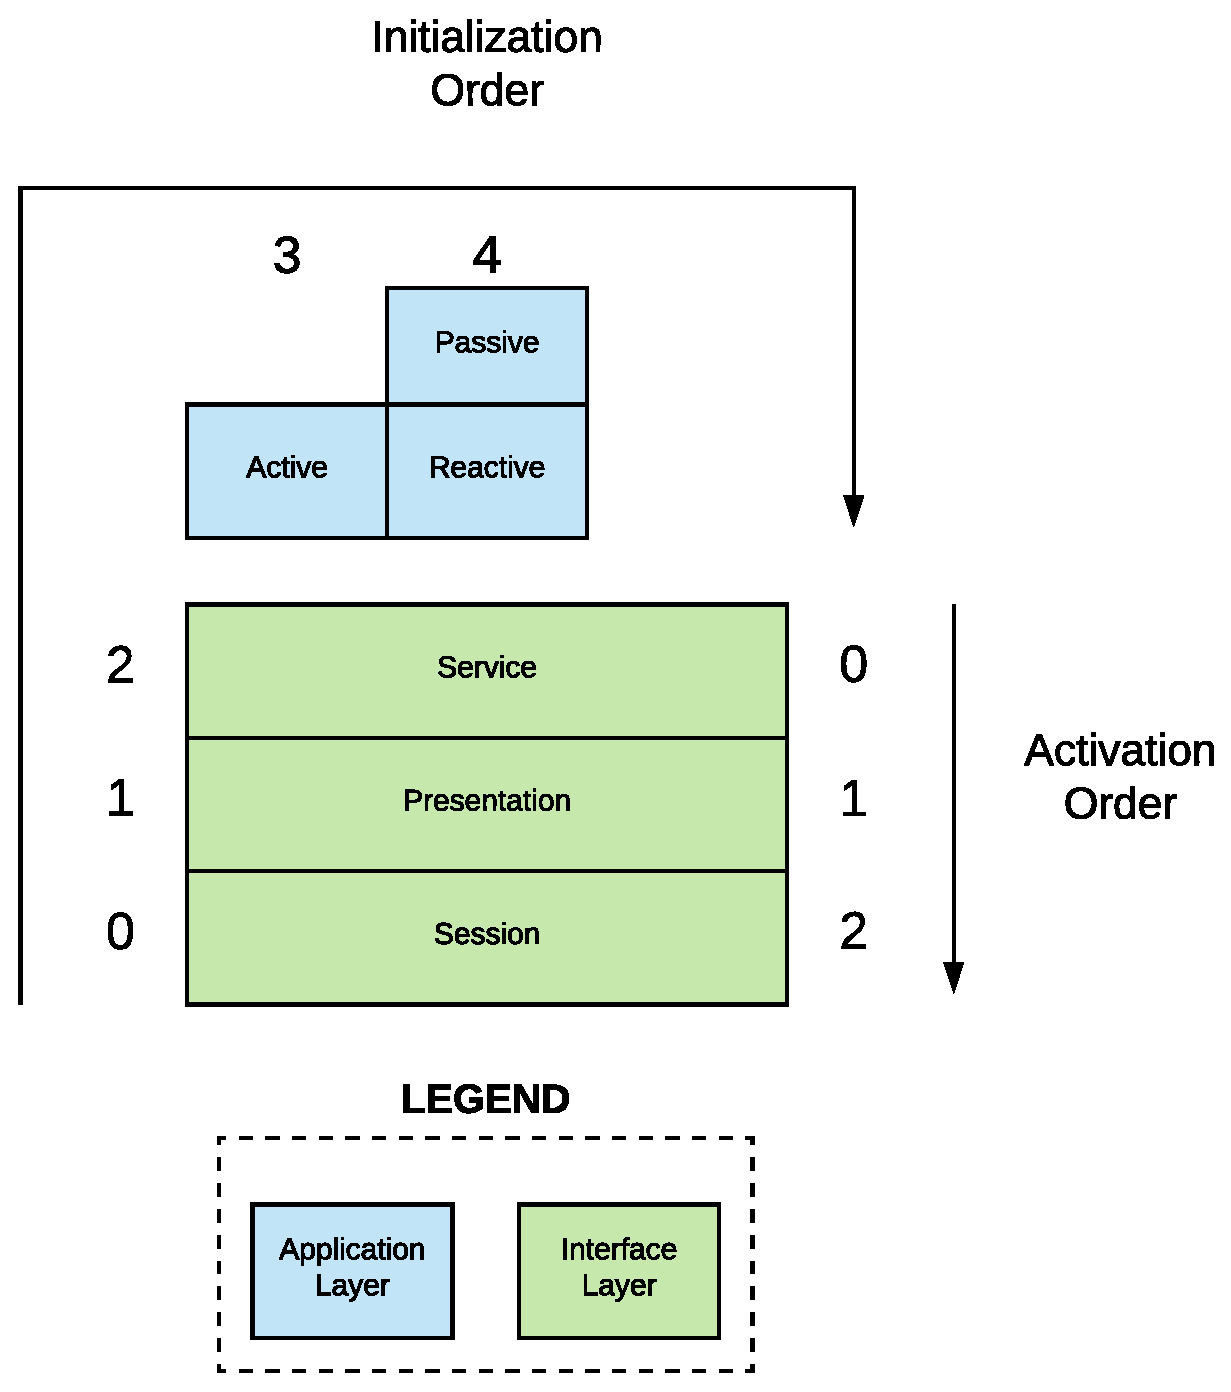
\includegraphics[scale=0.5,keepaspectratio]
    {images/solution/init_activate.eps}
  \caption{Application Bootstrap - Init}
  \label{fig:sd-app-init}
\end{figure}


\subsubsubsection{Init}

Each application node contains the \textit{Init} process,
which is the parent of all the application processes.
The execution steps of \textit{Init} are depicted in Figure
\ref{fig:sd-app-init}.
It instantiates the resources of each layer, thus making
Interface Layer and Application Layer transit from the \verb|inactive|
to the \verb|ready| state.
For example, each sublayer of Interface Layer instantiates its own pool of
LWPs\footnote{lightweight processes}.

The Application Layer initialization completes in the following order:

\begin{enumerate}
  \item \textbf{Active:} the entities which move in the city (e.g.,
    pedestrians);
  \item \textbf{Reactive:} the infrastructure of the city (e.g., streets);
\end{enumerate}

The Scheduling package, which manages the execution order for the events of the
Application Layer, does not require an initialization step. This package
will be started directly through the start message.


Since the \textit{Passive} entities are stateless and
logically belong to \textit{reactive} entities (e.g., speed limits belong to
roads), they will be instantiated along with them
(Figure \ref{fig:sd-entity-types-deps}).

When \textit{Reactive} completes its initialization, \textit{Init}
signals the Application layer completion to each sublayer of Interface Layer
in the following order:

\begin{enumerate}
  \item \textbf{Service:} provides activators and pipelines services to
    application layer;
  \item \textbf{Presentation:} provides data conversion services;
  \item \textbf{Session:} provides network connection services (e.g., senders
  and receivers).
\end{enumerate}

\textit{Init} triggers the transition of each IL sublayer state from
\verb|ready| to \verb|active|.
The activation order is extremely important to proactively avoid
message losses between remote nodes.
Indeed, at this stage, the application layer is
not able to generate or receive messages because the start message has not
been sent by the middleware. Obviously, IL is a reactive component
of the backend subystem. Thus, its \verb|active| state means
that all the workers of IL have started their event loop.
Their loop execution is triggered each time a
message arrives. Indeed, the workers are blocked on unbounded synchronized
queues which have been designed to be thread safe \cite{taft2006ada}.


The service and the presentation layer are activated before the session layer;
the latter exposes a remote communication channel through TCP
sockets.
Finally, the application is ready to communicate because both of its layers
has been activated.

Now, the Application waits the \verb|start|
message from the middleware.


A crash of the \textit{Init} process, occurring before the end of the
bootstrap, is detected by the middleware layer. The expiration
of a timeout triggers a retransmission from the middleware side.
Note that this model should also work for a bootstrap which is executed
starting
from a valid snapshot of the system, with the only difference consisting in
divergent values of the configuration file.
Indeed, for each simulation we will use a set
of configurations which is going to be different for each city.

\subsubsubsection{Start}

When \textit{Init} completes, the Application Layer is in a \verb|ready| state
while Interface Layer is in an \verb|active| state.
The first message sent by the middleware towards the Interface Layer is a
\verb|start| message which triggers the Application Layer activation.

The \verb|start| message kickoffs the scheduler, causing it to load the set
of actions declared in its configuration file. An action is a $<$\verb|agent|,
\verb|time_span|$>$ pair, i.e., the active entity \verb|agent| will act in
\verb|time_span| milliseconds.
